\part{Modeling of concurrent programs}
\section{Learning Goals}
\begin{itemize}
\item An understanding of how using message-based synchronization leads to a very different design than shared variable synchronization.
\item Model, in FSP and by drawing transition diagrams, simple programs (semaphore-based or message-passing).
\item Draw very simple compound (for parallel processes) transition diagrams.
\item  Sketch simple message-passing programs.
\item An understanding of how using message-based synchronization leads to fewer transition-diagram states than shared variable synchronization.
\item Understanding the terms deadlock and livelock in context of transition diagrams
\end{itemize}

\section{Modeling}
Classic deadlock example:
\begin{verbatim}
T1:
    while (1) {
        Wait(A)
        Wait(B)
        ...
        Signal(A)
        Signal(B)
    }
T2:
    while (1) {
        Wait(B)
        Wait(A)
        ... 
        Signal(B)
        Signal(A)
    }
\end{verbatim}
Let us introduce \textbf{processes} and \textbf{events}. All processes that 'care about' an event experience it at the same time. For modeling we use FSP (Finite State Processes) $\subset$ CSP (Communicating Sequential Processes). Note that Ada \texttt{entries} can be modelled as events.  For message-based systems (message passing, synchronous communication), modeling with processes, events and guards comes naturally. Some explanation of symbols before we get into the next part. The numbers below in the diagrams are the \textbf{states}. In the textual representation these are \textbf{arrows.} The text such as $t1sa$ is an event. What this means is that to get for example an $t1sa$ event, T1 process has to be in state 3 and SA process has to be in state 2. Check the diagrams below, this is a bit tricky but makes sense.
\begin{verbatim}
    T1 = (t1wa -> t1wb -> t1sb -> t1sa -> T1).
    T2 = (t2wb -> t2wa -> t2sa -> t2sb -> T2).
\end{verbatim}
\begin{figure}[H]
\centering
\begin{subfigure}{.5\textwidth}
\centering
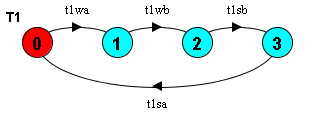
\includegraphics[width=.9\linewidth]{figures/Modeling concurrent programs/Example1/T1.PNG}
\end{subfigure}%
~
\begin{subfigure}{.5\textwidth}
\centering
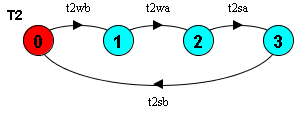
\includegraphics[width=.9\linewidth]{figures/Modeling concurrent programs/Example1/T2.PNG}
\end{subfigure}
\end{figure}

No deadlock is visible here, we need to model the semaphores:
\begin{verbatim}
    SA = (t1wa -> t1sa -> SA | t2wa -> t2sa -> SA).
    SB = (t1wb -> t1sb -> SB | t2wb -> t2sb -> SB).
\end{verbatim}
\begin{figure}[H]
\centering
\begin{subfigure}{.5\textwidth}
\centering
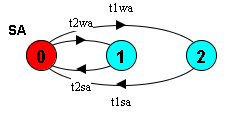
\includegraphics[width=.9\linewidth]{figures/Modeling concurrent programs/Example1/SA.PNG}
\end{subfigure}%
~
\begin{subfigure}{.5\textwidth}
\centering
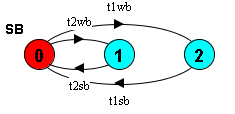
\includegraphics[width=.9\linewidth]{figures/Modeling concurrent programs/Example1/SB.PNG}
\end{subfigure}
\end{figure}
To model the complete, concurrent/parallel system:
\begin{verbatim}
    ||SYSTEM = (T1 || T2 || SA || SB).
\end{verbatim}
\begin{figure}[H]
    \centering
    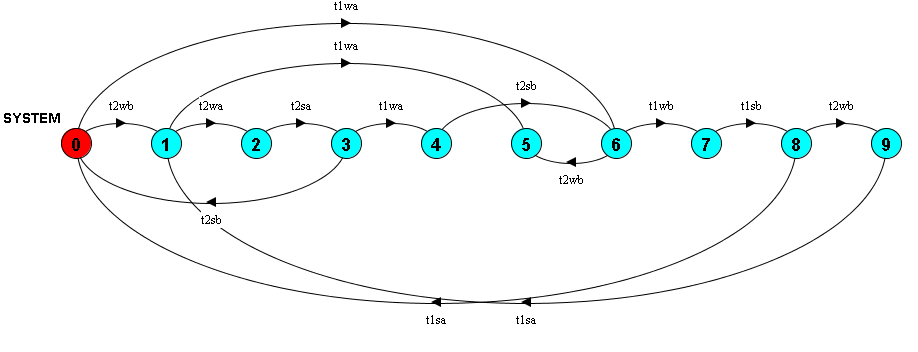
\includegraphics[width=\linewidth]{figures/Modeling concurrent programs/Example1/SYSTEM.PNG}
\end{figure}
In a \textbf{transition diagram}, a deadlock is a state with no exit. Such a state can be observed in the figure above in state 5. A livelock is a subset of states we cannot exit. 
\begin{verbatim}
LL = (s1 -> LOOP), LOOP = (s2 -> s3 -> LOOP).
\end{verbatim}
\begin{figure}[H]
\centering
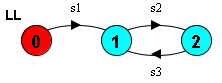
\includegraphics[width=0.5\linewidth]{figures/Modeling concurrent programs/LiveLock/LiveLock.PNG}
\end{figure}
Before mentioning the Dining philosophers problem, have a look at this basic code producing a deadlock
\begin{verbatim}
MOVE = (north->(south->MOVE|north->STOP)).
\end{verbatim}
\begin{figure}[H]
\centering
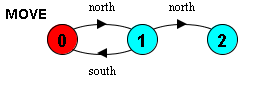
\includegraphics[width=0.5\linewidth]{figures/Modeling concurrent programs/Deadlock/Deadlock.PNG}
\end{figure}
Dining philosophers with deadlock is shown next
\begin{verbatim}
    FORK = (get -> put -> FORK).
    PHIL = (sitdown -> right.get -> left.get -> eat ->
            right.put -> left.put -> arise -> PHIL).
    
    || DINERS(N=5) = forall [i:0..N-1]
            (phil[i]:PHIL ||
            {phil[i].left, phil[(i-1+N)%N].right}::FORK).
\end{verbatim}
Some advance syntax is used here:
\begin{itemize}
    \item \texttt{phil[i]:PHIL} exchanges \texttt{eat} with \texttt{phil1.eat}, and thus takes care of all events for all N philosophers.
    \item \texttt{{phil[i].left, phil[(i-1+N)\%N].right}} means that either of the two options in curly braces are possible.
    \item \texttt{{phil[i].left, phil[(i-1+N)\%N].right}::FORK} then means that either \texttt{phil[i].left.get} or \texttt{phil[(i-1+N) mod N].right.get} are possible for the same fork, i.e. it can be picked up by the philosopher to its right or left.
\end{itemize}
Transition diagram is huge, needs an analyzing tool such as the infamous LTS Analyzer to find the deadlock potential! Some notes on the Dining Philosophers problem:
\begin{itemize}
\item If we make some of the philosophers left-handed the deadlock is avoided. But hugely unfair as one philosopher next to the one causing the deadlock would have to finish his meal before the other philosopher gets both his forks. \textit{This is not very well explained, sorry but I don't have a philosopher's stone that makes me godly enough to explain this well}
\item A a resource hierarchy on the forks, where the philosophers would always pick up the lowest value fork first could improve fairness. \textit{It is far beyond the scope of this compendium, this course, my sanity or the universe itself to properly explain why}
\end{itemize}
